\documentclass{report}

\usepackage{ugentstyle}
\usepackage{listings}

\begin{document}
	\maketitle{Beveiliging van netwerken en computers}
	\tableofcontents
	
	\part{Theorie}
	\chapter{Inleiding}
	Het woord \textit{security} kan verschillende betekenissen hebben, het is dan ook een zeer breed onderwerp. Concepten van security zijn onder andere: \textit{Authenticatie, autorisatie, encryptie, bitcoins, social engineering, malware, sociale media, ...}. Zelfs bij een goed beveiligd systeem zijn er nog altijd risicofactoren :
	\begin{itemize}
		\item de informatie kan nog altijd niet-digitaal gewisseld worden.
		\item de gebruikers zijn niet goed opgeleid.
	\end{itemize}
	Beveiliging is belangrijk aangezien dat informatie 
	\begin{itemize}
		\item waarde kan hebben
		\item gestolen of beschadigd worden
		\item vervalst kan worden.
	\end{itemize}
	\chapter{Basisconcepten}
	\section{Security Model}
	Een security model is een diagram waarop verschillende beveilingscomponenten met elkaar interageren.
	\section{Security Goals}
	Beveiling heeft een aantal doelen. Deze doelen kunnen zelden allemaal op hetzelfde moment gerealiseerd worden en vaak moet er een deel opgeofferd worden om de overige doelen te behalen.
	\begin{itemize}
		\item \textbf{Confidentialiteit.} De informatie mag enkel door de zender en ontvanger van een bericht gelezen worden. Dit wordt gerealiseerd door encryptie toe te passen, waarbij enkel de zender en ontvanger dit kunnen decrypteren aan de hand van een sleutel. Bij de basisvorm van confidentialiteit weet een aanvaller nog steeds dat er een bericht is verstuurd en wie de zender/ontvanger is. Een uitbreiding is verkeersconfidentialiteit dat tracht de zender en ontvanger onbekend te maken.
		\item \textbf{Authenticatie.} Dit is het proces dat nagaat of een persoon zegt wie hij is. Er zijn drie verschillende methoden.
		\begin{enumerate}
			\item \textit{Entiteit authenticatie.} Dit is het bewijzen aan de hand van bepaalde informatie zoals een e-mailadres of een uniek ID nummer.
			\item \textit{Attribute authenticatie.} Dit is een extra vorm van authenticatie die vaak toegepast wordt nadat entiteit authenticatie voltooid is. Dit soort authenticatie specialiseert de authenticatie op basis van een rol of functie.
			\item \textit{Data-origin authenticatie.} Het bewijzen dat de informatie van de juiste bron komt. 
		\end{enumerate}
	    Een slecht authenticatiesysteem kan in staat zijn dat personen zich kunnen voordoen als anderen. Het eisen van een digitale handteking die enkel door de echte persoon kan getekend worden is een oplossing.
		\item \textbf{Autorisatie.} Dit is het proces waarbij extra privileges toegekend worden aan reeds geauthenticeerde entiteiten op basis van een rol of functie.
		\item \textbf{Data integriteit.} Er moet een garantie zijn dat de verzonden en ontvangen data dezelfde is. Een oplossing is om een sequentienummer bij te houden in combinatie met een digitale handtekening. Dit sequentienummer moet voldoen aan bepaalde veiligheidsmaatregelen. Het sequentienummer dient om meervoudige versies van hetzelfde bericht te omzeilen.
		
		\item \textbf{Niet-verlorenbaarheid.} Het niet kunnen ontkennen dat een bepaal bericht verzonden of ontvangen werd. 
		
		\item \textbf{Beschikbaarheid.} De informatie moet beschikbaar zijn wanneer deze opgevraagd wordt. Aanvallen zoals een DDoS kan de beschikbaarheid verhinderen.
	\end{itemize}

	\section{Security Threats}
	Er zijn passieve aanvallen zoals eavesdropping en verkeeranalyse. Voorbeelden van actieve aanvallen zijn berichtwizigingen, hijacking en een DDoS. Er wordt onderscheid gemaakt tussen drie mogelijke aanvallen:
	\begin{enumerate}
		\item \textbf{Brute-force.} Deze manier van werken is niet realistisch.
		\item \textbf{Cryptoanalyse.} Het analyseren van een systeem om informatie of sleutels te bemachtigen.
		\item \textbf{Side-channel.} Gebruik maken van fysieke eigenschappen om informatie of sleutels te bemachtigen.
	\end{enumerate}
	\section{Security Mechanismen}
	\subsection{Encryptie}
	Het encrypteren van informatie is niets meer dan het vertalen van deze informatie met behulp van een algoritme (de sleutel). Informatie dat \textbf{symmetrisch} geëncrypteerd wordt gebruikt dezelfde sleutel voor het encrypteren als decrypteren. Een voorbeeld van zo een algoritme is de Caesar Cipher waarbij $E_n(x)$ de encryptie en $D_n(x)$ de decryptie voorstelt.
	$$E_n(x) = (x + n)\; mod\; 26 \qquad D_n(x) = (x - n)\; mod\; 26$$
	Probeer volgend stukje tekst te decrypteren met $n = 2$:
	\texttt{GCUA VQ DTGCM}. Het is dan ook duidelijk dat deze cipher niet echt veilig is aangezien er maar 26 mogelijkheden zijn. Die mogelijkheden afgaan is vrij realistisch met de hand te doen. Zelfs indien $n$ niet gegeven was bij bovenstaand voorbeeld waren twee iteraties voldoende om de gedecrypteerde tekst te achterhalen. 
	
	Een andere vorm is \textbf{assymetrisch} encrypteren. Dit princiepe maakt gebruik van een \textit{private} en een \textit{public} sleutel. De private sleutel van een gebruiker G is enkel gekend door G zelf. G zal, indien hij een bericht verstuurd, deze sleutel gebruiken om dit bericht te encrypteren. Ontvangt hij echter een bericht, zal hij deze sleutel gebruiken om dit bericht te decrypteren. De publieke sleutel voor G is gekend door alle andere gebruikers. Andere gebruikers gebruiken deze publieke sleutel om berichten te encrypteren zodat G deze kan decrypteren met zijn private sleutel.
	
	\subsection{Hashing}
	Een hashfunctie \textbf{H(m)} genereert een hash \textbf{h} voor een gegeven input \textbf{m}. Een hashfunctie dat gebruikt wordt voor beveiliginsdoeleinden moet aan een aantal vereisten voldoen:
	\begin{itemize}
		\item Het moet werken voor elke lengte van m.
		\item Ze moeten berekening snel uitvoeren. Hier kan een uitzondering op gemaakt worden indien de hashfunctie deel uitmaakt van heel gevoelige informatie zoals paswoorden. Een tragere hashfunctie zal aanvallers ook vertragen.
		\item Het moet een \textbf{one-way} functie zijn. Dit wil zeggen dat, indien \textbf{h} gegeven is, \textbf{m} onmogelijk te achterhalen moet zijn.
		\item Er moet \textbf{weak collision resistance} zijn. Het moet onmogelijk zijn om een bericht \textbf{n} te genereren zodat \textbf{H(n) = H(m)}. Is dit niet het geval, kan het mogelijk zijn dat er totaal andere data verstuurd kan worden door een aanvaller, maar die data heeft dezelfde hash als de geldige data. De ontvanger zal niet doorhebben dat hij met foutieve informatie werkt. Integriteit en data-origin authentication worden hier overtreden.
		\item Er moet ook \textbf{strong collision resistance} zijn. Indien \textbf{n} een bericht is dat verschillend is van \textbf{m}, mag de hashfunctie nooit dezelfde \textbf{h} uitkomen voor deze twee inputs. Indien dit wel mogelijk is, kan een aanvaller meerdere versies van een document genereren die dezelfde hashwaarde hebben. Niet-verlorenbaarheid wordt hier overtreden.
	\end{itemize}
	Strong collision resistance is veel moeilijker om te implementeren dan weak collision resistance. De kans dat twee berichten uit een groep van \textbf{k} berichten dezelfde hashwaarde opleveren met een hashfunctie die \textbf{N} waarden kan genereren is: 
	$$P(N, k) = \frac{1 - N!}{((N - k)! N^k)} = 1 - e^{\frac{-k^2}{2N}}$$
	hieruit volgt 
	$$k \approx -\sqrt{N} \ln(1 - P(N, k))$$
	Stel nu \textbf{P(N, k)) = 0.99}, dan is \textbf{k $\approx$ 4,6} en \textbf{$\sqrt{N} \approx 4,6 \cdot 2^{n/2}$}.
	\subsection{Message Authentication Code}
	Een \textbf{Message Authentication Code (MAC)} kan net zoals een hash gebruikt worden om informatie te encrypteren. De input van deze functie is echter een combinatie van plaintext en een geheime sleutel. Het biedt ook bijkomende functionaliteit:
	\begin{itemize}
		\item Controle of een bericht aangepast wordt.
		\item Controle of dat de verzender correct is
		\item Indien een sequentienummer bijgehouden wordt, dat de berichtvolgorde gerespecteerd wordt.
	\end{itemize}

	\textbf{MAC} kent een gelijkenis met \textbf{symmetrische encryptie}. In beide gevallen moet de zender en ontvanger een geheime sleutel hebben zodat ze hetzelfde authenticatiemechanisme hebben. Het nadeel is natuurlijk dat de ontvanger ook deze sleutel moet hebben. MAC biedt wel geen confidentialiteit. Dit laat echter toe om beide functies op te splitsen. De authenticatie kan met een MAC gebeuren op een server, terwijl confidentialiteit de taak is van een werkstation, gebruik makend van encryptie. Gegeven de notatie \textbf{$MAC = C_k(M)$} met k de geheime sleutel en M het bericht. Een MAC moet aan volgende vereisten voldoen:
	\begin{itemize}
		\item Indien $M$ en $C_k(M)$ gekend zijn, moet het onmogelijk zijn om een bericht $M'$ te construeren zodat \textbf{$$C_k(M') = C_k(M)$$}. Dit is nodig voor data-integriteit
		
		\item De waarden die $C_k(M)$ kan aannemen met gelijk verspreidt worden over alle mogelijke waarden van de MAC. De kans dat twee berichten $M$ en $M'$ dezelfde MAC krijgen moet $\frac{1}{2^n}$ zijn.
	\end{itemize}

	De ideale MAC is enkel kwetsbaar voor brute force aanvallen. 

	\chapter{Netwerk en communicatiebeveiliging}
	\section{SSH}
	\textbf{Secure Shell (SSH)}biedt een client-server toepassing en encrypteert uitwisselingen tussen de twee. Verder biedt SSH volgende functioneleiten ook aan:
	\begin{itemize}
		\item Tunneling. TCP verkeer kan getunneld worden door een SSH connectie.
		\item Bestandoverdracht met \textbf{Secure Copy (SCP} en \textbf{SSH File Transfer Protocol (SFTP)}.
		\item X-session forwarding en port forwarding.
		\item Maakt gebruik van geteste algoritmen voor encryptie, data-integriteit, sleuteluitwisseling en publieke sleutel management. De sleutels voor encryptie moeten ten minste 128 bits zijn.
	\end{itemize}
	\subsection{SSH Transport Layer Protocol}
	De transportlaag is verantwoordelijk voor sleuteluitwisselingen en server authenticatie. Het garandeert confidentialiteit en integriteit en forward privacy. Dit wil zeggen dat, indien een sleutel door een aanvaller gekend is gedurende een sessie, zullen vorige sessies niet in gevaar zijn. Een server kan meerdere hosts keys hebben die op zich verschillende asymmetrische encryptietechnieken gebruiken. Meerdere hosts kunnen dezelfde hosts key gebruiken. Om authenticatie mogelijk te maken, moet een client de publieke sleutel van de server kennen. Hiervoor bestaan er twee mogelijkheden (zoals gespecificeerd in \textbf{RPF 4251}:
	\begin{itemize}
		\item De client heeft een lokale database dat elke host name met een public host key zal associëren. Hierdoor is er geen centrale entiteit nodig. Het nadeel is dat de database lastig is om te onderhouden.
		\item Een host name-to-key associatie is gecertificeerd door een \textbf{Certification Authority (CA)}. De client kent enkel de CA root key en kan de geldigheid van alle host keys die geaccepteerd zijn door de CA nagaan. Het voordeel is hier dat de client slechts één sleutel moet bijhouden. Het nadeel is dat een host eerst moet gecertificeerd worden voor dat authorisatie mogelijk wordt.
	\end{itemize}
	Een client en server gaan een algoritme onderhandelen om de encryptie mee uit te voeren. Dit verloopt in volgende stappen:
	\begin{enumerate}
		\item Leg een TCP verbinding tussen de server en de client.
		\item De client zal zijn versie van SSH doorsturen in de vorm van \texttt{SSH-protoversion-softwareversion} waarbij de server zal reageren met zijn versie. Dit is nodig aangezien sommige versies incompatiebel zijn met elkaar.
		\item De client stuurt een lijst van ondersteunde methoden voor elke categorie algoritmen in de lijst: sleuteluitwisseling, encryptie, MAC algoritme en compressie.
		De server kiest voor elke categorie het algoritme dat hij ook ondersteunt en de voorkeur krijgt door de client.
		\item De sleuteluitwissling vindt nu plaats. \todo{todododod}
	\end{enumerate}
Pakketten die met SSH verstuurd worden hebben volgend formaat:
	\begin{itemize}
		\item \textbf{Packet length}: De lengte in bytes, zonder de lengte van het pakket lengte veld (4 bytes) en het MAC veld.
		\item \textbf{Padding length}: De lengte van het random padding veld.
		\item \textbf{Payload}: Dit bevat de eigenlijke informatie van het pakket. Dit kan eventueel gecompresseerd worden indien compression gewenst is door de client. Het maximale aantal bytes van het payload veld is 32768 bytes.
		\item \textbf{Random padding}: Nadat een encryptiealgoritme genegotieerd wordt, zal dit veld toegevoegd worden. Het bevat een willekeurig aantal bytes (4 tot 255) waarmee het pakket uitegbreid wordt zodat de pakketlengte een veelvoud is van de cipher block size. Dit is nodig om cryptoanalyse moeilijker te maken. Berichten die relatief een klein aantal bytes groot zijn hebben hier vooral een voordeel bij.
		\item \textbf{MAC}: Indien message authentication genegotieerd wordt, zal dit veld een MAC waarde krijgen. De MAC waarde wordt berekend over het hele pakket, exclusief het MAC veld, plus een extra sequentienummer. Het sequentienummer is een 32-bit getal dat met 1 geïncrementeerd wordt voor elk pakket. Dit sequentienummer wordt niet gereset indien de algoritmen zouden veranderen voor een SSH connectie.
	\end{itemize}
	Heel het pakket, exlusief het MAC veld, wordt ook nog geëncrypteerd en geauthenticeerd. Het encryptiealgoritme wordt zoals vermeld in het sleuteluitwisselingsproces bepaalt. Een algoritme dat zeker ondersteund moet worden is \textbf{3des-cbc}. Dit algoritme gebruikt een sleutelgrootte van 168 bits. Een aanbevolen algoritme is \textbf{aes128-cbc}. Het MAC algoritme wordt tijdens hetzelfde proces bepaalt. Twee verplichte ondersteunde algoritmen zijn \textbf{hmasc-sha1} en \textbf{hmac-sha1-96}. 
	\subsection{SSH User Authentication Protocol}
	Dit protocol zal de client authenticeren aan de server en bevindt zich ook op de transportlaag. Er zijn drie belangrijke authenticatiemethoden:
	\begin{itemize}
		\item \textbf{Password Authentication}: Dit is de meest eenvoudigste methode waarbij de client enkel een paswoord zal moeten meegeven. Dit paswoord is uiteraard beschermt via encryptie door het SSH Transport Layer Protocol.
		\item \textbf{Host Based Authentication}: In dit geval is de authenticatie gebaseerd op de host van een gebruiker. Een host kan meerdere gebruikers ondersteunen. De client verstuurt een handtekening die gegenereerd werd met de geheime sleutel van de client host. De server moet dus enkel de identiteit van de client host verifiëren en gaat ervan uit dat de authenticatie op de clientside correct verlopen is.
		
		\item \textbf{Public Key Authentication}: Een client verstuurd een bericht naar de server met de publieke sleutel van die client, waarbij het bericht getekend wordt door de client zijn geheime sleutel. Wanneer de server dit bericht ontvangt, zal deze eerst kijken of de publieke sleutel correct is, en daarna of dat de handtekening correct is. Indien ja, is de client geauthenticeerd op de server.
	\end{itemize}
	\subsection{Local Forwarding}


	\subsection{SSH Connection Protocol}
	\todo{snap ik niet}
	
	\textbf{Port Forwarding} heeft als doel een onveilige TCP verbinding om te vormen tot een veilige SSH verbinding. Dit wordt ook wel een SSH tunnel genoemd. Er bestaat een verschil tussen \textbf{lokaal} en \textbf{remote} forwarding. 
	\begin{itemize}
		\item \textbf{Local Port Forwarding (outgoing tunnel)}: Local Forwarding geeft aan dat een bepaalde poort op het lokale toestel geforward moet worden naar een bepaalde host en poort op een remote toestel. Het meest eenvoudige commando ziet er zo uit:
		\begin{lstlisting}
		ssh -L sourcePort:forwardToHost:onPort connectToHost
		\end{lstlisting}
		Dit betekent letterlijk: \textit{Connecteer met ssh naar connectToHost, en forward alle connecties op het lokaale sourcePort naar onPort van het toestel forwardToHost}. De parameters connectToHost en forwardToHost kunnen dezelfde zijn.	
		
		\item \textbf{Remote Port Forwarding}: Dit doet het omgekeerde als Local Forwarding. Een poort van een remote host zal geforward worden naar het client toestel. Hier moet de optie -L vervangen worden door -R. De parameters blijven dezelfde.
	\end{itemize}

	\part{Labo}
	\chapter{Routing + DNS}
	De bedoeling van dit labo is een netwerkconfiguratie op te stellen en een DNS-server op te zetten die je in latere labo's nog zal gebruiken. Zorg er dus voor dat je de configuratie waar mogelijk persistent maakt, en eventueel de nodige commando's in scripts opneemt zodat je tijdens volgende labo's de opstelling snel kan herstellen.  Vooraleer aan de instellingen van de (fysieke) labotoestellen iets te veranderen maak je een volledige backup van de \textbackslash etc directory (tar -cvjf \textbackslash root \textbackslash backup\_etc.tar.bz2 \textbackslash etc).
	Editeer geen enkel configuratiebestand zonder er eerst een kopie van te maken!
	
	Voor dit labo werken we met groepjes van twee studenten. Iedere groep zal zich ontfermen over één DNS-domein dat vier hosts omvat (twee fysieke toestellen en twee virtuele machines). Ieder fysiek toestel zal dus als host fungeren voor één virtuele machine. Figuur \ref{fig:opstelling} geeft een algemeen overzicht van de opstelling voor één groep.
	\begin{figure}
		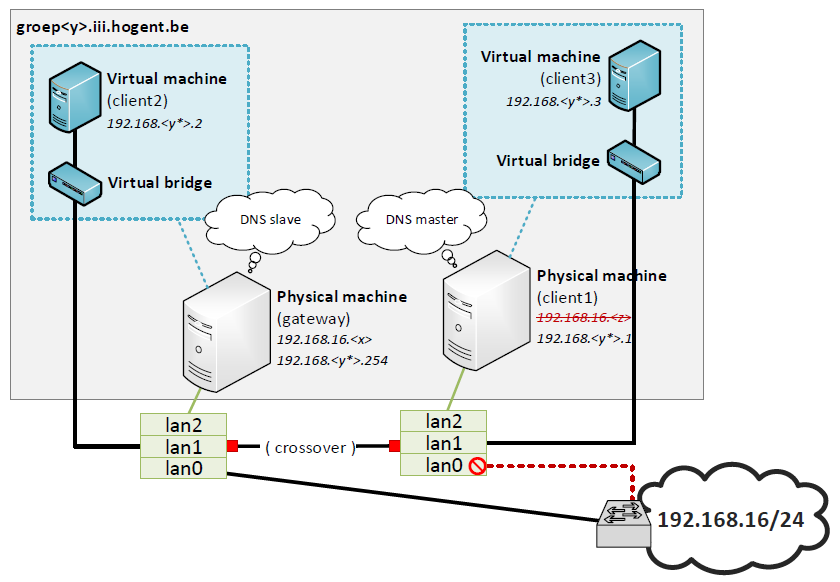
\includegraphics[width=\textwidth]{opstelling}
		\caption{Opstelling}
		\label{fig:opstelling}
	\end{figure}
	Voor de uitwerking van dit labo wordt de groep op figuur \ref{fig:groep} gebruikt.
	\begin{figure}
		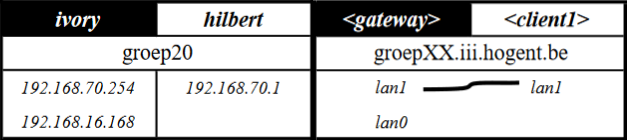
\includegraphics[width=\textwidth]{groep}
		\caption{Een groep}
		\label{fig:groep}
	\end{figure}
\section{Routing}
 Voor elke groep bestaat de opstelling uit vier verschillende hosts:
\begin{itemize}
	\item \textbf{gateway}: deze verbindt het interne netwerk van jouw groep met het HoGent netwerk via onze gateway 192.168.16.8. Dit toestel is via een crosskabel (lan1) verbonden met de tweede fysieke machine (client1).
	\item \textbf{client1}: deze is via een crosskabel (lan1) verbonden met de gateway. Merk op dat dit toestel niet rechtstreeks verbonden is met het HoGent netwerk!
	\item \textbf{client2}: dit is een virtuele machine die draait op de gateway. Deze virtuele machine is via een virtuele bridge verbonden met het interne netwerk (lan1) van de gateway.
	\item \textbf{client3}: dit is een virtuele machine die draait op client1. Deze virtuele machine is via een virtuele bridge verbonden met het interne netwerk (lan1) van client1.
	
\end{itemize}
\subsection{Configuratie IP-adressen}
Voor de netwerkconfiguratie maak je overal gebruik van statische IP-adressen (ook voor lan0 op de gateway). Om te testen kan je eerst gebruikmaken van het \textit{ip} commando, maar uiteindelijk is het eenvoudigst om een configuratiebestand te voorzien per interface. De configuratiebestanden vind je bij Fedora terug in de folder \texttt{/etc/sysconfig/network-scripts/}. 
\begin{itemize}
	\item \textbf{Gateway}: \begin{itemize}
								\item \texttt{ifcfg-lan0}:
									  		\begin{lstlisting}
DEVICE=lan0
BOOTPROTO=none
ONBOOT=yes
NETMASK=255.255.255.0
IPADDR=192.168.16.168
GATEWAY=192.168.16.8
											\end{lstlisting}
								\item \texttt{ifcfg-lan1}:
\begin{lstlisting}
DEVICE=lan0
BOOTPROTO=none
ONBOOT=yes
NETMASK=255.255.255.0
IPADDR=192.168.70.254
\end{lstlisting}											
							\end{itemize}
	\item \textbf{Client1}: 
	\begin{itemize}
		\item \texttt{ifcfg-lan1}:
		\begin{lstlisting}
DEVICE=lan1
BOOTPROTO=none
ONBOOT=yes
NETMASK=255.255.255.0
IPADDR=192.168.70.1
GATEWAY=192.168.70.254
		\end{lstlisting}										
	\end{itemize}

	\item \textbf{Client2}: 
\begin{itemize}
	\item \texttt{ifcfg-enp0s3}:
	\begin{lstlisting}
DEVICE=enp0s3
BOOTPROTO=none
ONBOOT=yes
NETMASK=255.255.255.0
IPADDR=192.168.70.2
GATEWAY=192.168.70.254
	\end{lstlisting}										
\end{itemize}

	\item \textbf{Client3}: 
\begin{itemize}
	\item \texttt{ifcfg-enp0s3}:
	\begin{lstlisting}
DEVICE=enp0s3
BOOTPROTO=none
ONBOOT=yes
NETMASK=255.255.255.0
IPADDR=192.168.70.3
GATEWAY=192.168.70.254
	\end{lstlisting}										
\end{itemize}

\end{itemize}

\subsection{OSPF}

Op de gateway gebruik je OSPF om de route naar jouw subnet te multicasten. Als router-software maak je gebruik van quagga en twee zelfgemaakte configuratiebestanden zebra.conf en ospfd.conf die je in de directory \texttt{/etc/quagga} plaatst. Aangezien iedere gateway rechtstreeks verbonden is met het 192.168.16.0/24 netwerk laten we dit overeenstemmen met area 0. Het is dus niet nodig om bijkomende areas in het leven te roepen!
Ken aan je interfaces geen IP-adressen toe via quagga maar doe dit dus op de traditionele manier met het commando ip of via ifcfg-files.
Vergeet niet om routing actief te zetten op de nodige hosts.
Om te testen of je configuratie werkt, moet je zowel de zebra daemon als de ospfd daemon starten. 

\begin{itemize}
	\item \textbf{zebra.conf}:
		\begin{lstlisting}
hostname ivory
password pass
enable password pass
log stdout
!
interface lan0
!
interface lan1
!
		\end{lstlisting}
	\item \textbf{ospfd.conf}:
		\begin{lstlisting}
hostname ivory
password pass
enable password pass
log stdout
!
interface lan0
!
interface lan1
!
router ospf
	redistribute connected
	network 192.168.16.0/24 area 0.0.0.0
!
\end{lstlisting}

\end{itemize}
Voeg \texttt{net.ipv4.ip\_forward = 1} toe aan het bestand \texttt{/etc/sysctl.conf}. 
Voer nu het commando \texttt{systemctl status/restart/enable zebra/ospfd} uit. \textit{Restart} zal de daemon herstarten en \textit{enable} geeft aan dat de daemon bij de bootprocedure moet opgestart worden. Met \textit{status} kan nagegaan worden of dat de configuratie correct verlopen is.
\section{DNS}
Binnen de opstelling configureer je ook twee DNS-servers die verantwoordelijk zijn voor het subdomein van de groep (groep20.iii.hogent.be). \textbf{client1} doet dienst als primaire (master) DNS-server, de \textbf{gateway} als secundaire (slave) DNS-server. Binnen je domein voorzie je zowel een forward als een reverse DNS lookup zone. Alle aanvragen die niet voor jouw domein bedoeld zijn stuur je via een \textbf{forwarder} door naar 192.168.16.8. 
\subsection{Configuratie named}
 Wij hebben reeds voor jou een DNS-root-server geconfigureerd. Bijgevolg kunnen alle DNS-aanvragen die geen betrekking hebben op jouw domein doorgestuurd worden naar 192.168.16.8. Dit is ook de default-gateway van de router en moet als dusdanig worden ingesteld. Jouw DNS-server voorziet in de naamgeving voor de vier hosts in het domein. Om voldoende redundantie te hebben, configureer je op de gateway een secundaire nameserver.

Voor DNS maken we gebruik van de BIND/named service die reeds op de fysieke toestellen geïnstalleerd is. De configuratie moet je zelf nog aanpassen of aanmaken. Maak hiervoor gebruik van volgende directories en bestanden:

\begin{itemize}
	\item \texttt{/etc/named.conf}: algemene configuratie BIND/named.
	\item \texttt{/var/named/}: zonebestanden voor jouw domein
\end{itemize}


Om te testen of het configuratiebestand en de zonebestanden correct zijn, kan je respectievelijk gebruikmaken van de \texttt{named-checkconf} en \texttt{named-checkzone} commando's. Eenmaal de configuratie correct is, kan je de named service (her)starten via het systemctl commando.
Voor de virtuele machines gebruik je als hostname de naam van je toestel, gevolgd door 'VM'. De virtuele machine op computer Kronecker zal bv. de naam KroneckerVM hebben.
Voorzie zowel een forward als een reverse DNS lookup zone die de vier hosts bevat en test grondig uit! Aangezien veel services die we tijdens de labo's gebruiken steunen op reverse DNS, is het belangrijk dat deze correct geconfigureerd is. 
\begin{itemize}
	\item \textbf{/etc/named.conf}: 
	\begin{itemize}
		\item client1:
			\begin{lstlisting}
options {
	directory	"/var/named";
	dump-file	"/var/named/data/cache_dump.db";
	statistics-file	"/var/named/data/named_stats.txt";
	memstatistics-file "var/named/data/named_mem_stats.txt";
	allow-query	{ any; };
	recursion yes,
	empty-zones-enable no;
	forwarders { 192.168.16.8; };
};

logging {
	channel default_debug {
		syslog daemon;
		severity dynamic;
	}
};

zone "groep20.iii.hogent.be" IN {
	type master;
	file "groep20.iii.hogent.be";
	allow-transfer { 192.168.70.254; };
};

zone "70.168.192.in-addr.arpa" {
	type master;
	file "70.168.192.in-addr.arpa";
	allow-transfer { 192.168.70.254; };	
};

			\end{lstlisting}
		\item gateway: 
		\begin{lstlisting}
options {
	directory	"/var/named";
	dump-file	"/var/named/data/cache_dump.db";
	statistics-file	"/var/named/data/named_stats.txt";
	memstatistics-file "var/named/data/named_mem_stats.txt";
	allow-query	{ any; };
	recursion yes,
	empty-zones-enable no;
	forwarders { 192.168.16.8; };
};

logging {
	channel default_debug {
		syslog daemon;
		severity dynamic;
	}
};

zone "groep20.iii.hogent.be" IN {
	type slave;
	file "groep20.iii.hogent.be";
	masters { 192.168.70.254; };
};

zone "70.168.192.in-addr.arpa" {
	type slave;
	file "70.168.192.in-addr.arpa";
	masters { 192.168.70.254; };
};
		\end{lstlisting}
	\end{itemize}
	\item \textbf{/var/named/groep20.iii.hogent.be}
	\begin{lstlisting}
$TTL 60
@ IN SOA groep20.iii.hogent.be. bert.desaffel.ugent.be (1 60 1H 60 3H)
  IN NS	 hilbert
hilbert 	IN	A	192.168.70.1
hilbertVM 	IN	A	192.168.70.3
ivory 		IN	A	192.168.70.254
ivoryVM	 	IN	A	192.168.70.4
	\end{lstlisting}
	\item \textbf{/var/named/70.168.192.in-addr.arpa}
	\begin{lstlisting}
$TTL 60
@   IN SOA 70.168.192 bert.desaffel.ugent.be (1 60 1H 60 3H)
    IN NS hilbert.groep20.iii.hogent.be.	
1   IN PTR hilbert.groep20.iii.hogent.be.
3   IN PTR hilbertVM.groep20.iii.hogent.be.
2   IN PTR ivoryVM.groep20.iii.hogent.be.
254 IN PTR ivory.groep20.iii.hogent.be.
	\end{lstlisting}	
\end{itemize}

\subsection{Clientconfiguratie}
Alle hosts moeten gebruikmaken van de eigen DNS-servers, hiervoor pas je \texttt{/etc/resolv.conf} aan. Voeg aan dit bestand ook een optie toe om de verschillende DNS-aanvragen over beide nameservers te verdelen.
Zorg er voor dat DHCP uitgeschakeld is (BOOTPROTO=none in de ifcfg-files) voor elke netwerkinterface van de host! Indien dit niet het geval is, zal de dhcp-client bij elke herstart de inhoud van het /etc/resolv.conf bestand overschrijven.

Bovendien stel je ook op elk van de 4 clients de juiste hostname in, maak hierbij gebruik van de Fully Qualified Domain Name (FQDN). Om de hostname in te stellen kan je gebruikmaken van onderstaande commando's. 
\begin{lstlisting}
hostnamectl set-hostname --static <name>.groep20.iii.hogent.be
hostnamectl set-hostname --transient <name>.groep20.iii.hogent.be
hostnamectl set-hostname --pretty <name>.groep20.iii.hogent.be
\end{lstlisting}
Op alle vier de toestellen in \texttt{/etc/resolv.conf}:
\begin{lstlisting}
domain groep20.iii.hogent.be
nameserver 192.168.70.1
nameserver 192.168.70.254
options rotate
\end{lstlisting}
\section{Uittesten}
 Vooraleer de opstelling af te breken test je deze grondig uit! Eventueel kan je ook alle machines eens herstarten, om na te gaan of de configuratie volledig persistent is.
	
	Uiteindelijk moet je vanaf elke host alle toestellen binnen het eigen netwerk kunnen bereiken. Dit kan je eenvoudig testen via het ping commando. Bovendien moet je vanaf elke host ook onze gateway (192.168.16.8) kunnen bereiken, alsook alle toestellen van de andere groepen binnen het lokaal. Een ping pakket sturen naar buiten (bv. ping google.be) heeft weinig zin, aangezien de firewall van de HoGent alle ICMP-pakketten blokkeert.
	
	Om je DNS-server te testen kan je gebruikmaken van het dig commando. Test je DNS-servers kritisch uit, en probeer ook of je het domein van je buren kan bereiken. 

\chapter{SSH}
 Voor dit deel maak je gebruik van de virtuele machines die je in het vorige labo hebt aangemaakt. Maak vooraf een zip van de virtuele harde schijf die je na afloop van het labo terugplaatst. Wijzig in geen geval de configuratiebestanden van de fysieke toestellen.

Het aanpassen van de configuratie en het herstarten van de server doe je als root-gebruiker.
Het configureren en uitvoeren van de de client-commando's doe je meestal als een gewone gebruiker (tiwi1, ...), soms als root indien nodig. Maak daarom bij het begin van dit labo 3 extra gebruikers aan op je virtuele machine: tiwi1, tiwi2 en tiwi3 (zelfde wachtwoord als root). 
\begin{lstlisting}
(in de command shell)
adduser tiwi1
passwd tiwi1 
root
adduser tiwi2
passwd tiwi2
root
adduser tiwi3
passwd tiwi3
root
\end{lstlisting}
Om in te loggen met een gebruiker: \texttt{su - tiwi1}
\section{Host Based Authentication}
 SSH laat toe om host-based authentication te doen, zodat een specifieke gebruiker op een specifieke host kan inloggen zonder wachtwoord. Om Host-Based Authenticatie te gebruiken moet je zowel de \textbf{/etc/ssh/sshd\_config} (server) als de \textbf{/etc/ssh/ssh\_config} (client) moeten aanpassen, en zal je eveneens de nodige informatie moeten toevoegen aan \textbf{~/.ssh/known\_hosts} en \textbf{~/.shosts}.

Zorg er voor dat je toegang kunt krijgen/geven voor een gebruiker op een andere machine via Host-Based Authentication.
Test dit uitgebreid uit! Dit effect kan ook verkregen worden door een globale serverinstelling en niet door gebruik te maken van een .shosts-file voor de gebruiker. Configureer dit en test uit voor zowel root als voor een gewone gebruiker. 
\begin{itemize}
	\item \textit{Vm van hilbert (client)}
		\begin{itemize}

			\item Volgende lijn aanpassen in \textbf{ssh\_config}:
			\begin{lstlisting}
HostBasedAuthentication yes
EnableSSHKeysign yes
			\end{lstlisting}
			\item Genereer een sleutelpaar met 
			$$\texttt{ssh-keygen -t rsa -f /etc/ssh/ssh\_host\_rsa\_key -N '' ''}$$
		\end{itemize}
	\item \textit{VM van ivory (server)}
		  \begin{itemize}
		  	\item Volgende lijnen aanpassen in \textbf{sshd\_config}:
		  		\begin{lstlisting}
HostBasedAuthentication yes
IgnoreRhosts no
IgnoreUserKnownHosts no
RHostsRSAAuthentication yes
		  		\end{lstlisting}
		  	\item Genereer een \textbf{known\_hosts} bestand door 
		  		$$\texttt{ssh root@hilbert.groep20.iii.hogent.be}$$
		  		in te geven. Er zal een waarschuwing komen dat hij een entry zal toevoegen. Het is belangrijk dat de sshclient dit bestand zelf genereerd zodat de rechten onmiddelijk goed zijn. Na het genereren moet de publieke sleutel van de client toegevoegd worden aan dit bestand. Gebruik hiervoor volgend commando:
		  		$$\texttt{ssh-keyscan -t rsa hilbert.groep20.iii.hogent.be >> .ssh/known\_hosts}$$
		  		
		  	\item De Fully Qualified Domain Name (FQDN) van de client moet toegevoegd worden in het \textbf{.shosts} bestand. Dit kan eenvoudig door 
		  	$$\texttt{echo hilbert.groep20.iii.hogent.be >> ~/.shosts}$$
		  	uit te voeren. De rechten van dit  bestand worden best aangepast zodat enkel de eigenaar schrijfrechten heeft. 
		  	$$\texttt{chmod og-w ~/.shosts}$$
		  \end{itemize}

\end{itemize}
\end{document}

